\chapter{Asking Millionaire Homeowners How They Got Rich}

This chapter is built from a field report rather than a blackboard lecture. We begin at gates, in driveways, beside cars, and inside living rooms, and the conceptual work of the episode lies in the repeated mechanisms that emerge beneath the spectacle: risk, reinvestment, tax drag, fast decisions, belief transfer, pressure, and reserve-building. Since there is no validated boardwork to preserve, we formalize only what the transcript clearly supports and keep the speaker's order of discovery intact.

\section{Wealth as a Field Site in Los Angeles}

The lecture opens by turning visible wealth into a search problem. The host approaches luxury homes and frames Los Angeles as a city in which wealth is sufficiently concentrated that repeated visits may reveal repeated principles. In the lecture's own terms, the city is introduced by the claim
\begin{equation}
\operatorname{rank}_{\text{millionaires}}(\text{Los Angeles}) = 6.
\end{equation}
This is a framing statistic, not a theorem proved on the page. Its function is methodological. It tells us why the host is moving through Bel-Air, Beverly Hills, and Calabasas rather than speaking in abstractions: the lecture wants to sample success where it is presumed to be densely visible.

The rhythm of the opening matters. We first see a gate, an intercom, luxury cars, and the ordinary social friction of asking strangers for access. Only after this visible hook does the host widen the frame to the city and then narrow it again to a specific question: what did these homeowners actually do, and what can a younger person borrow from that path to wealth in 2023?

The result is a useful narrative stance for the whole chapter. We are not yet being given a theory of wealth. We are being shown a procedure for finding one.

\section{Risk, Self-Belief, and Real-Estate Building}

The first successful interview gives the lecture its first genuine model. The speaker says she was once a model, then moved into renovating homes, and then into building homes. The host asks first for duration, then for industry, and only after the biographical foundation is in place does the interview turn to advice. The sequence is exact and should be preserved: career transition first, general principle second.

Her explicit principle is simple: take a risk, believe in yourself, and believe in what you do. In a weaker lecture that would remain a slogan. Here the host presses for scale by asking for the largest amount of money generated in a single year on a property. The answer is concrete:
\begin{equation}
\Pi_{\text{last property}} = \$3.5\times 10^6.
\end{equation}
At this point the lecture changes character. It is no longer enough to say that risk matters. Once a number appears, the next question must ask how one number becomes a repeatable process.

The case closes, for the moment, with advice aimed at the younger generation: hard work, focus, and a stable goal. But before the chapter returns to those closing imperatives, it correctly pauses over the scaling problem.

\subsection{Question \& Answer}

\paragraph{Question.} How does one profitable deal become scalable wealth rather than a single exceptional year?

\paragraph{Answer.} The speaker's answer is iterative. Profit is not mainly consumed; it is rolled into the next build. The lecture states this in ordinary language, but the logic can be written cleanly as an update rule for deployable capital:
\begin{align}
K_1 &= K_0 + \Pi_0,\\
K_2 &= K_1 + \Pi_1 = K_0 + \Pi_0 + \Pi_1,\\
K_n &= K_0 + \sum_{j=0}^{n-1}\Pi_j.
\end{align}
Here \(K_n\) denotes the capital available for the next project after project \(n\), and \(\Pi_n\) denotes the profit generated by project \(n\). The point is not that every \(\Pi_n\) is equal, or even that each project must succeed. The point is that a successful cycle enlarges the next starting point.

In this lecture the growth loop is said twice, once informally and once economically: reinvest over and over, and the projects get larger and larger. A compact schematic of that logic is useful.

\begin{figure}
\centering
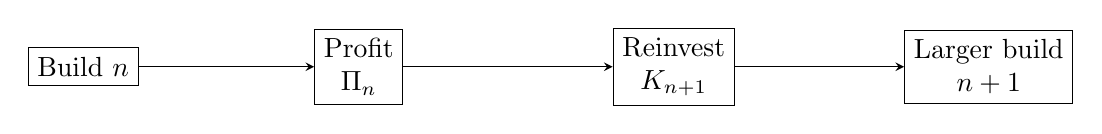
\begin{tikzpicture}[>=stealth]
\node[draw, rectangle, align=center] (b0) at (0,0) {Build $n$};
\node[draw, rectangle, align=center] (p) at (3.5,0) {Profit\\$\Pi_n$};
\node[draw, rectangle, align=center] (r) at (7.5,0) {Reinvest\\$K_{n+1}$};
\node[draw, rectangle, align=center] (b1) at (11.5,0) {Larger build\\$n+1$};
\draw[->] (b0) -- (p);
\draw[->] (p) -- (r);
\draw[->] (r) -- (b1);
\end{tikzpicture}
\end{figure}

The lecture then names one specific instrument: the 1031 exchange. No detailed tax law is derived, and we should not pretend otherwise. But the comparative effect stated in the interview is clear:
\begin{equation}
K_{n+1}^{(\text{tax deferred})} > K_{n+1}^{(\text{immediate tax})}.
\end{equation}
That inequality captures the full strategic content needed here. If less capital leaks out between projects, then more capital enters the next build, and the recurrence steepens.

\begin{remark}
The lecture uses the 1031 exchange only as a practical tax-deferral device. Nothing in the transcript justifies a technical treatment beyond the simple comparative statement that rolling gains forward leaves more money inside the next project.
\end{remark}

Now the interview can close as it began, with advice addressed downward in age and outward in audience. Hard work, focus, and the refusal to stop are no longer floating aphorisms. They stand at the end of a process that has already been partially formalized.

\section{Rejection, Reset, and Entrepreneurial Longevity}

After the first interview, the lecture does something structurally important. It interrupts its own success. We are sent back into the street and shown refusals, privacy, gatekeepers, and the host's frustration. This is not dead air. It restores the cost of access and keeps the chapter from becoming a frictionless anthology of wealthy people saying wise things.

The next accepted case arrives in a different register. The host flags that the speaker was driving a Porsche; the interview itself then shifts quickly to biography and survival in business. The speaker says he started in software engineering, moved into marketing, and has run his agency for nine years:
\begin{equation}
\tau_{\text{agency}} = 9\ \text{years}.
\end{equation}
The host places the conceptual obstacle sharply: if \(90\%\) of businesses do not make it, what prevents entrepreneurial longevity from collapsing under ordinary mistakes and disappointments?

The answer is practical, sequential, and strikingly unsentimental. The speaker says he ran a startup, failed to build the multi-billion-dollar company he wanted, and even though the company was acquired, he did not treat that outcome as the intended victory. The lesson is not triumphalism. It is the refusal to turn a local failure into a permanent verdict on the self.

We can summarize the logic of this passage as a persistence-and-decision heuristic:
\begin{enumerate}
\item A setback occurs.
\item One does not convert the setback into a total judgment on oneself.
\item One keeps moving forward instead of freezing.
\item One makes the next decision quickly.
\item One returns to execution before overthinking can harden into paralysis.
\end{enumerate}
This is exactly the place in the lecture where speed of decision appears as a commercial variable. The speaker explicitly says that one of the biggest things helping him in his career has been fast decision-making. The reason is easy to see: time lost in self-doubt compounds just as surely as capital does.

The section ends with a lighter question about owning a Porsche one day, but even that beat serves a structural purpose. The dream object is not treated as pure vanity. It is attached to work, investment, saving, and long memory. The host then recaps the speaker as a software engineer turned marketing multimillionaire, and the episode is ready for its largest and most elaborate case.

\section{Influence, Faith, and the Architecture of Scale}

The Calabasas segment begins with the same visual grammar as the opening: a large house, expensive cars, and the question of what work could have produced such a position. But the lecture quickly turns from display to biography. The speaker says he was born, in the transcript's rendering, in ``Columbia,'' came to the United States at age six, and then watched the family dream become a nightmare when the home was raided and both parents went to jail. At ten he makes a promise to care for the house. At fifteen he becomes, in effect, head of household.

This is not ornamental narrative. It prepares the next move. The lecture wants the architecture of scale to appear as a response to pressure rather than as a sterile management theory. Once the personal background is established, the business frame becomes quantitative:
\begin{align}
\tau_{\text{home security}} &= 25\ \text{years}, &
\tau_{\text{solar}} &= 1.5\ \text{years},\\
\operatorname{rank}_{\text{Inc5000}}(\text{solar company}) &= 20, &
R_{\text{this year}} &= \$2.0\times 10^8.
\end{align}
These are the figures that justify the host's scaling question. If the current year is projected at two hundred million dollars, the lecture is obliged to ask what principle converts hustle into organized scale.

The first answer is influence. To attract good people, the speaker says, those people must believe in you. This is a social version of capitalization. A dream must be large enough that other people's ambitions can fit inside it. The lecture does not yet formalize that thought, but it will soon give us the key term that makes it operational.

\subsection{Question \& Answer}

\paragraph{Question.} What does ``faith'' mean in business terms?

\paragraph{Answer.} The lecture defines it with unusual precision: faith is taking action before you have what you need. The example is concrete. The speaker bought the minivan before the people had arrived to fill it. In cautious notation, we may write
\begin{equation}
a_t > 0 \qquad \text{while} \qquad r_t < r^\ast,
\end{equation}
where \(a_t\) is a committed action, \(r_t\) is presently available resource, and \(r^\ast\) is the imagined threshold of readiness.

The speaker's claim is that the usual order is wrong. One does not wait for full readiness and then act. One acts, and the act itself produces a new internal state. The logic runs as follows:
\begin{enumerate}
\item A concrete commitment is made before the full resource set is visible.
\item The commitment converts intention into cost.
\item Cost raises what the speaker calls the necessity level.
\item Higher necessity raises urgency.
\item Higher urgency draws out latent ability and forces organization.
\item The missing people and capacities are then assembled under pressure.
\end{enumerate}
This is the operational content of the lecture's line that low stress is low performance. It should not be stated as a theorem of human nature, but within the argument of the interview it names an entrepreneurial technique: create enough commitment that comfort is no longer an option.

The same section then turns from action to persuasion. The speaker says he validated his business for himself by reading about home invasions and fire accidents, thereby filling himself with belief in the value of what he was selling. This gives us a second compact relation:
\begin{equation}
c_A > c_B \;\Rightarrow\; \mathcal{I}(A\to B)\text{ favors }A.
\end{equation}
The equation is editorial, but the transcript supports it closely. The more certain person influences the less certain person. The deeper point is that sales, in this account, is not merely the transmission of information. It is the transfer of settled conviction.

Once that is clear, the earlier remarks about influence also sharpen. A large company is not scaled only by adding headcount or revenue. It is scaled by creating a field in which other people willingly place their own effort.

\section{Money Discipline, Motivated Ambition, and the Family Tree}

The lecture's last major movement narrows from nine-figure growth to household discipline. This narrowing is essential. It prevents the chapter from ending in pure charisma. After influence, faith, urgency, and sales, the speaker is asked for the best financial advice he has ever received. His answer is strikingly plain: split the check three ways.

If \(C\) denotes one incoming check or income event, then the rule may be written
\begin{align}
C &= C_{\text{live}} + C_{\text{tax/sav}} + C_{\text{reserve}},\\
C_{\text{live}} &\approx C_{\text{tax/sav}} \approx C_{\text{reserve}} \approx \frac{C}{3}.
\end{align}
The lecture's force lies not in the algebra but in the prohibition attached to it. The reserve account is to be treated as if it does not exist. That behavioral fiction is what makes it real at the only moment that matters: the moment of pain.

The speaker explicitly says that life and pain are inseparable. The reserve account therefore functions as stored resilience. It is not a decorative extra; it is the financial counterpart of the earlier urgency doctrine. In one place the lecture says that pressure draws out hidden ability. Here it says that prior discipline softens future shocks. Together these form a coherent commercial temperament: commit hard, but also pre-build survival.

The section becomes more subtle when it turns to luxury. Nice things are not rejected. The speaker says he liked nice things, wanted to stand out, wanted to be rare, and wanted, at twenty-one, to be the first in his city driving a Mercedes convertible. In another register this would sound like vanity. Here it is presented as controlled fuel. Ambition is not denied; it is bounded by the three-bucket rule so that aspiration does not dissolve into ruin.

The final line of the episode gives the chapter its broadest social horizon: you do not come from a rich family, but a rich family can come from you. This is the correct ending. The lecture does not finally care about the car, the gate, or even the revenue figure. It cares about a repeated structure of decision that can change the direction of a household over generations.

\section{Summary}

The chapter begins with spectacle but does not remain there. First we are shown wealth as a field of inquiry. Then the first real-estate case gives us risk, self-belief, a profit figure, and a reinvestment loop strengthened by tax deferral. The rejection montage restores friction, after which the Porsche interview isolates a different variable: longevity depends on continued motion and fast decisions after disappointment. The Calabasas case then deepens the theory of scale by introducing influence, pre-commitment, faith as action before readiness, and certainty as a force in sales. Finally, the lecture descends from large-company growth to a simple money rule: split the check, protect the reserve, and let ambition remain a servant rather than a master.

If we strip the episode to its durable mathematical skeleton, it is this: capital compounds when profit is rolled forward, organizations grow when commitment precedes comfort, persuasion works when conviction is internally settled, and families change when disciplined allocation is repeated long enough. That is the lecture's commercial spine, and it is why the narrative order matters so much. The host does not tell us the formula first. He walks us to it.